\documentclass[conference]{IEEEtran}
\IEEEoverridecommandlockouts
% The preceding line is only needed to identify funding in the first footnote. If that is unneeded, please comment it out.
\usepackage{cite}
\usepackage{amsmath,amssymb,amsfonts}
\usepackage{algorithmic}
\usepackage{graphicx}
\usepackage{textcomp}
\usepackage{xcolor}
\usepackage{subfigure}
\usepackage{url}
\usepackage{lipsum}
\def\BibTeX{{\rm B\kern-.05em{\sc i\kern-.025em b}\kern-.08em
    T\kern-.1667em\lower.7ex\hbox{E}\kern-.125emX}}
\begin{document}

\title{Ghost Towns: Web Community Health Analysis}

\author{\IEEEauthorblockN{1\textsuperscript{st} Heng Jerry Quan}
\IEEEauthorblockA{\textit{CMPE 256} \\
\textit{SJSU}\\
San Jose, USA \\
heng.j.quan@sjsu.edu}
\and
\IEEEauthorblockN{2\textsuperscript{nd} Andrew Selvia}
\IEEEauthorblockA{\textit{CMPE 256} \\
\textit{SJSU}\\
San Jose, USA \\
andrew.selvia@sjsu.edu}
\and
\IEEEauthorblockN{3\textsuperscript{rd} Sean Wu}
\IEEEauthorblockA{\textit{CMPE 256} \\
\textit{SJSU}\\
San Jose, USA \\
shao-an.wu@sjsu.edu}
}

\maketitle

\begin{abstract}
Quickly compressing the web's scale and heterogeneity into similar communities is an ideal task for large-scale analytic techniques. This project employs the Label Propagation Algorithm to extract communities from web crawl data. These communities are then fed into a post-processing system which identifies websites which are no longer accessible. Communities composed of a large number of inaccessible websites are labeled "ghost towns". Taken holistically, this project demonstrates how to evaluate the health of web communities at scale.
\end{abstract}

\begin{IEEEkeywords}
Large-scale Analytics, Community Detection, Label Propagation
\end{IEEEkeywords}

\section{Introduction}

One of the Internet's core advantages is its openness. It enables the distribution of free speech at unprecedented scale. Of course, this property also leads to chaos. Making sense of such a large corpus of information is not trivial. Luckily, decades of concerted effort and research have manifested in tools and techniques for processing this information graph.

This project leverages the expertise of others in the fields of web archival, graph community detection, and distributed computing. Its primary aim is to analyze the health of web communities. In this context, the health of a web community is defined as the proportion of sites within a community which are accessible.

\subsection{Related Work}

The primary inspiration which led to this research is the "Large-scale Graph Mining with Spark" work performed by Win Suen. In her articles, she describes how to detect communities from web archives using label propagation and Apache Spark. Her general approach is leveraged, though many of the gaps are fleshed out with complete implementations. Additionally, a post-processing phase for determining the liveness of sites within a community is introduced.

\section{Tools and Techniques}

\subsection{Community Detection}

Approaches like hierarchical clustering, k-means clustering, and label propagation can be employed to detect communities. This project focuses on label propagation due to its built-in support within GraphFrames: a graph processing library built atop Apache Spark.

The combination of Spark and GraphFrames enables rapid iteration. Spark provides distributed data processing, critical when working with large-scale web archive data. GraphFrames, built directly upon Spark's DataFrame API, elevates this project further my handling all the core graph representation duties. Furthermore, it provides a ready-made implementation of the Label Propagation Algorithm.

\subsection{CommonCrawl Data}

CommonCrawl provides free, off-the-shelf web crawl data dating back 7 years. Access is simple since the entire dataset is hosted on AWS S3. One need only choose a month's web crawl and a subset to retrieve. The results described in this paper utilize a single file from the February 2020 crawl.

Importantly, CommonCrawl vends the data in Web Archive (WARC) format. This highly-compacted representation encodes a full request and response transaction for each URL visited during the crawl. Though efficient for storage and transmission, WARC demands special care to process.

\subsection{Preparer}

Data preparation responsibilities are apportioned to Preparer: a novel application which takes raw WARC data as input and outputs communities derived from LPA. Custom-built for this project, it is the primary integration point. It is written in Scala and built with SBT.

Raw WARC data is processed via ArchiveSpark: software which enables "efficient data processing, extraction, and derivation for archival collections", most-commonly web archives. Preparer utilizes its APIs for converting WARC data to CDX format. This translation taps into ArchiveSpark's primary advantage: performance. By pre-processing WARC data into CDX format (which only retains metadata), ArchiveSpark is able to perform common operations much faster than if raw WARC data was fed through Spark directly \cite{generatingCdx}.

After pre-processing, ArchiveSpark's enrichment functions \cite{enrichmentFunctions} are composed into a functional interface which is then applied over the web archive records. The resulting enrichment extracts all links in the HTML response body for an individual WARC record \cite{linkExtraction}. These links are further refined by stripping away all details from the path except the DNS name. For instance, https://example.com/api/123 would become just example.com. This step simplifies community detection later on.

Each DNS name pair will soon represent an edge in the graph. First, however, the DNS names are flattened distinctly into an RDD and each is assigned a hash ID. These IDs represent the vertices in the graph. The edges are simply mapped to their IDs before being finalized.

With vertices and edges defined, Preparer is now able to leverage GraphFrames to construct a graph. Finally, the LPA implementation provided via GraphFrames is invoked with a maximum iteration value of five. Whether it converges (not guaranteed) or reaches its fifth iteration, LPA will detect communities within the graph by iteratively grouping neighbors which share a common label. In the end, each vertex will be assigned to a label which hopefully aggregates similar sites by considering the links emanating from each. Preparer performs one final operation which groups the vertices by label and sorts each community by size in descending order.

Effort was expended to package Preparer in a single fat jar so it could be run via spark-submit on the SJSU HPC. Unfortunately, even provisioned with two nodes possessing 128GB RAM, Preparer repeatedly hit the timeout limit. Thankfully, it can be operated locally. The results in this paper are derived from a local execution of Preparer which took on the order of one hour to complete. Certainly, given more time for research, the SJSU HPC would be a more efficient environment in which to operate Preparer.

In conclusion, Preparer satisfies its contract of processing raw WARC data through a pipeline which includes LPA to detect communities. Though inspired by Win Suen's process, this procedure is truly novel as her data preparation code is excluded from her report and makes no mention of ArchiveSpark.

\subsection{Reaper}

TODO
\subsubsection{Version 2}
The first version of HTTP request system was a serialized version, 
which means if there exists on website link that does not respond in time the speed of the script will be slowed down, 
therefore parallel task distribution is need. 
Since the sequence of the output by the script does not matter, 
a Python concurrent futures library was used in this study; 
as HTTP header requests are I/O bound task, 
with ThreadPoolExecutor in use with the max workers set to 15 and connection timeout set to 3 seconds the speed of HTTP header requests can be boosted up to 350 URLs per minute.
 Moreover, in order to eliminate false negatives, 
another similar script was deployed with slight difference: 
With ThreadPoolExecutor in use with the max workers set to 3 and connection timeout set to 60 seconds, but only requests the URLs that were first seemed downed by the first script. By applying this method, 
it is observed that approximately 50\% of the false negatives were eliminated. 
Yet there are a total of 140k URLs so other faster tool is needed for the research.
\subsection{Visualization}

Running the LPA algorithm yielded about 20,000 different communities. These results are then visualized using the iGraph module in Python. Figure X.a shows a qualitative visualization of community size. A quick inspection indicates that there are many small communities and only a few large communities. Figure X.b confirms this numerically. Over half of all communities consist of only one website. Although the largest community has around 15,000 websites, the average community size is 6.3 websites, and the median community size is 2 websites.

\begin{figure}[htbp]
 \centerline{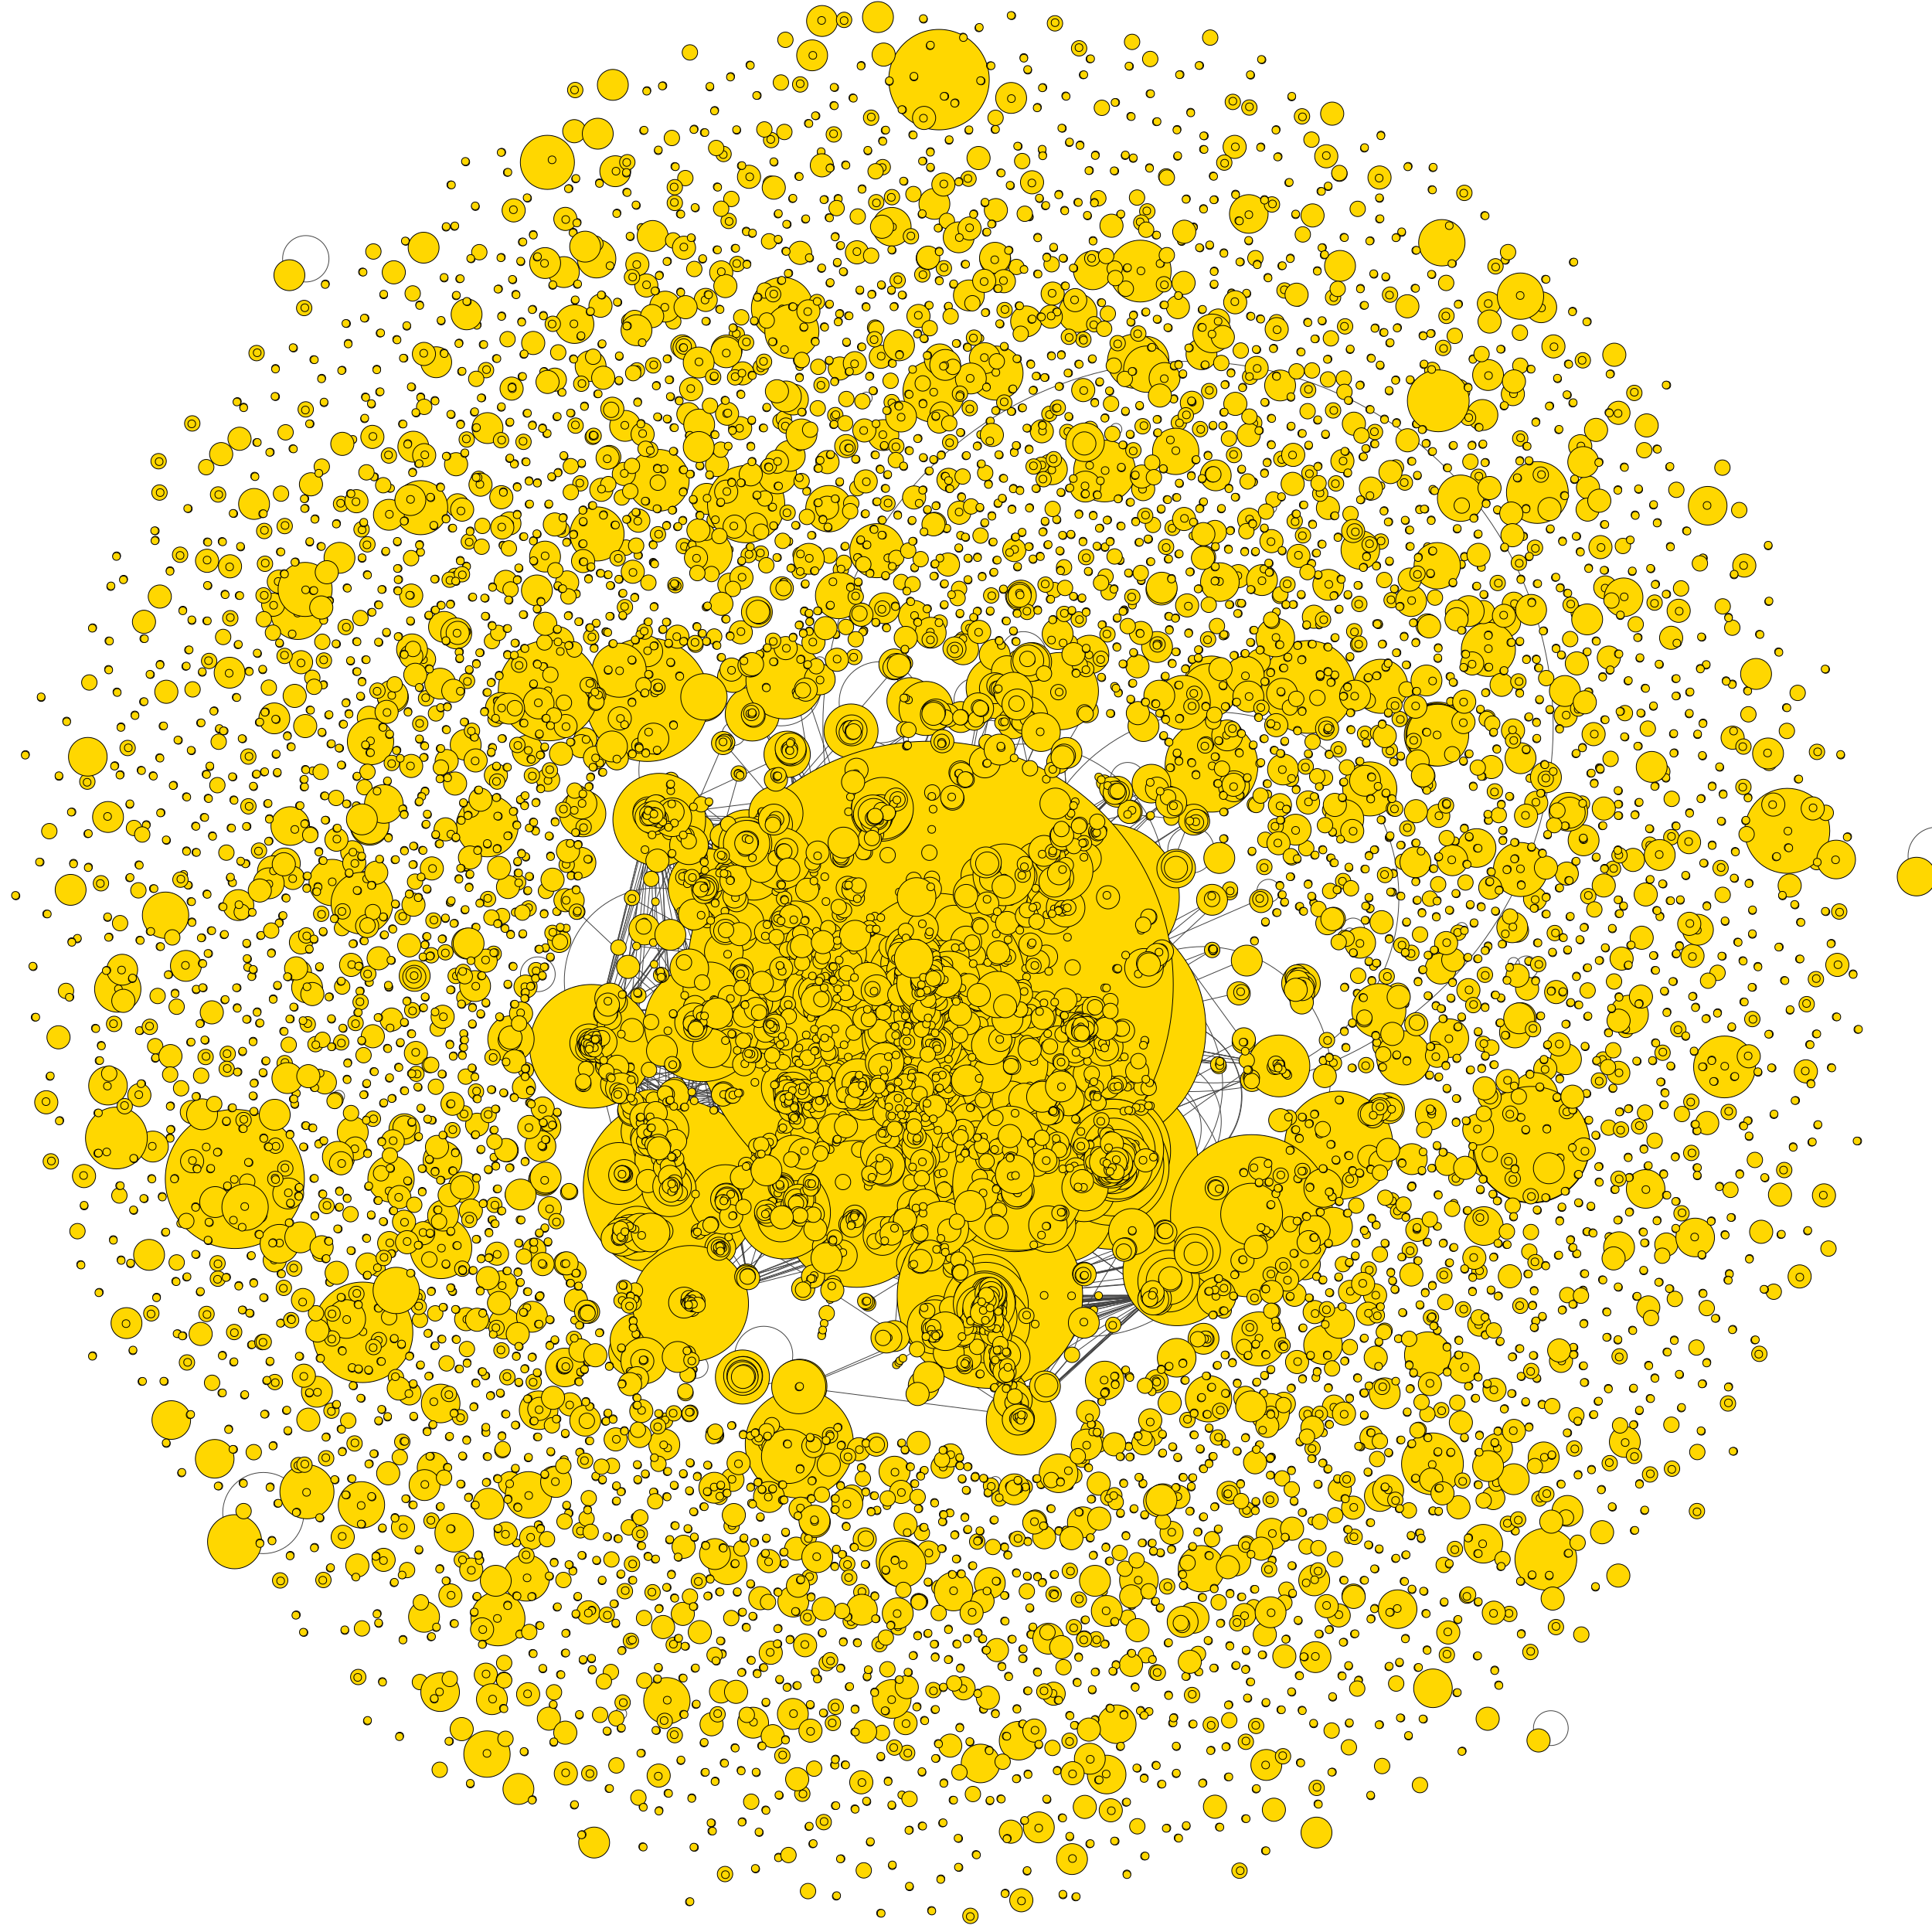
\includegraphics[width=\columnwidth]{communities_by_size.png}}
 \caption{Communities plotted by size; circle size and community size are directly proportional}
\end{figure}

\begin{figure}[htbp]
 \centerline{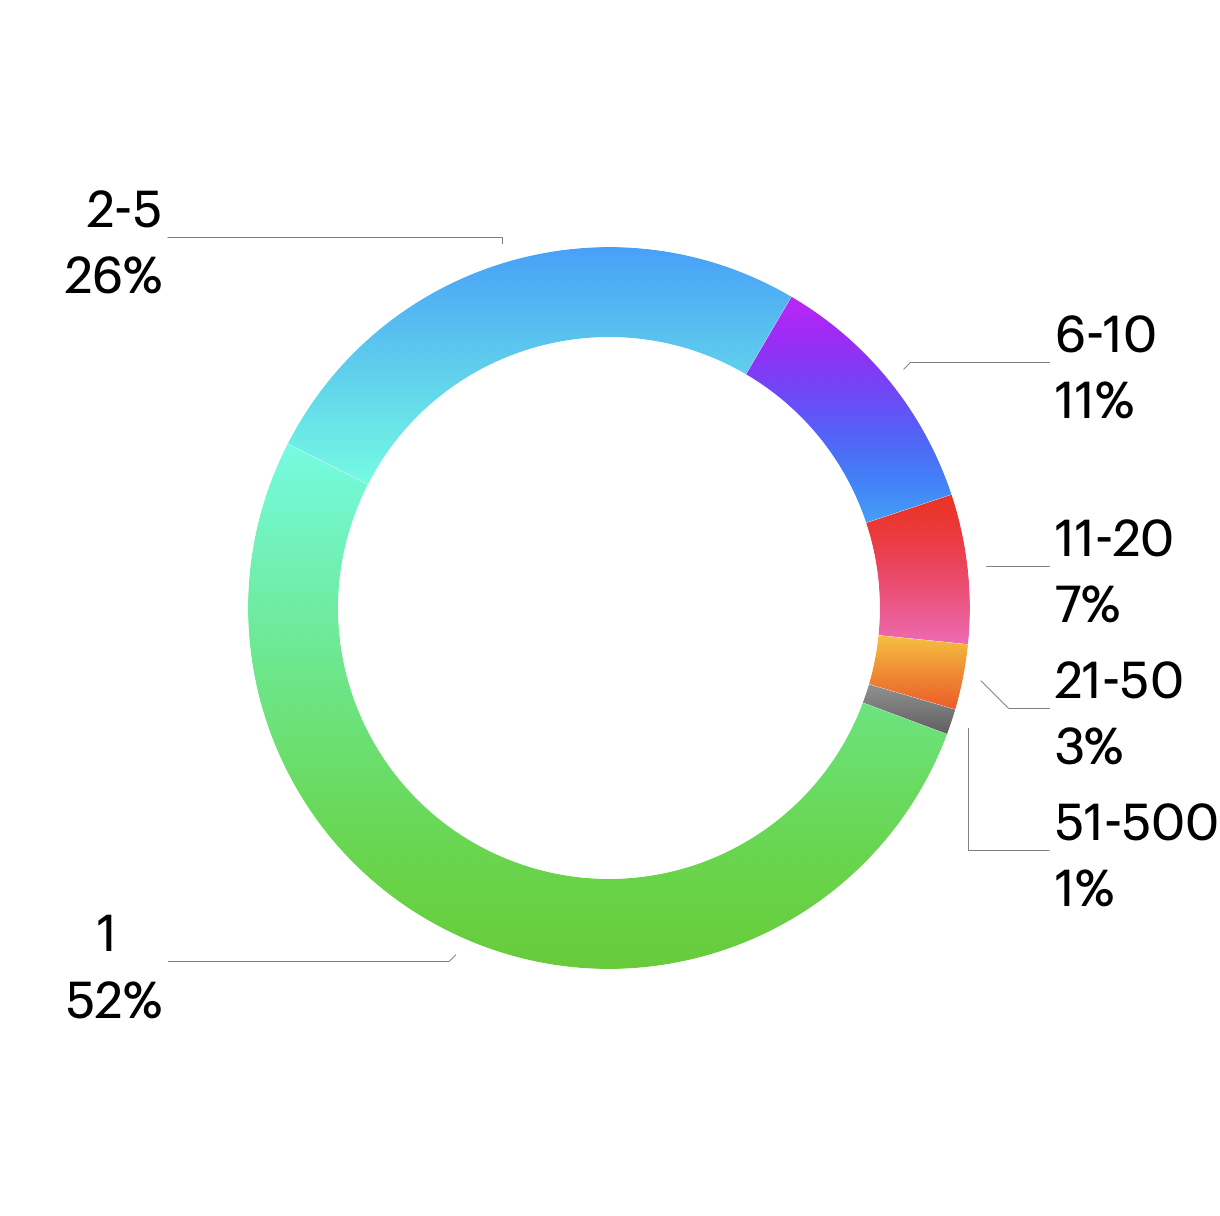
\includegraphics[width=\columnwidth]{CommunitySizeDistribution.png}}
 \caption{The distribution of community sizes detected by LPA.}
\end{figure}

On the individual community level, website statuses can be included in the graph. Websites that are down are represented by red nodes while sites that are still up are represented by green nodes. iGraph supports many different graph formats, and some formats visualize HTTP statuses more effectively while other formats are better at showing edges. Figure X2 visualizes the same community in two different layouts. The “circle” layout (Figure X2.a) is very good at displaying website statuses. The reader can get a good idea of the percentage of websites still up. When it comes to modeling the relationships between websites, however, the Fruchterman-Reingold layout \cite{fruchterman1991graph}(Figure X2.b) does a much better job.

\begin{figure}[htbp]
 \centerline{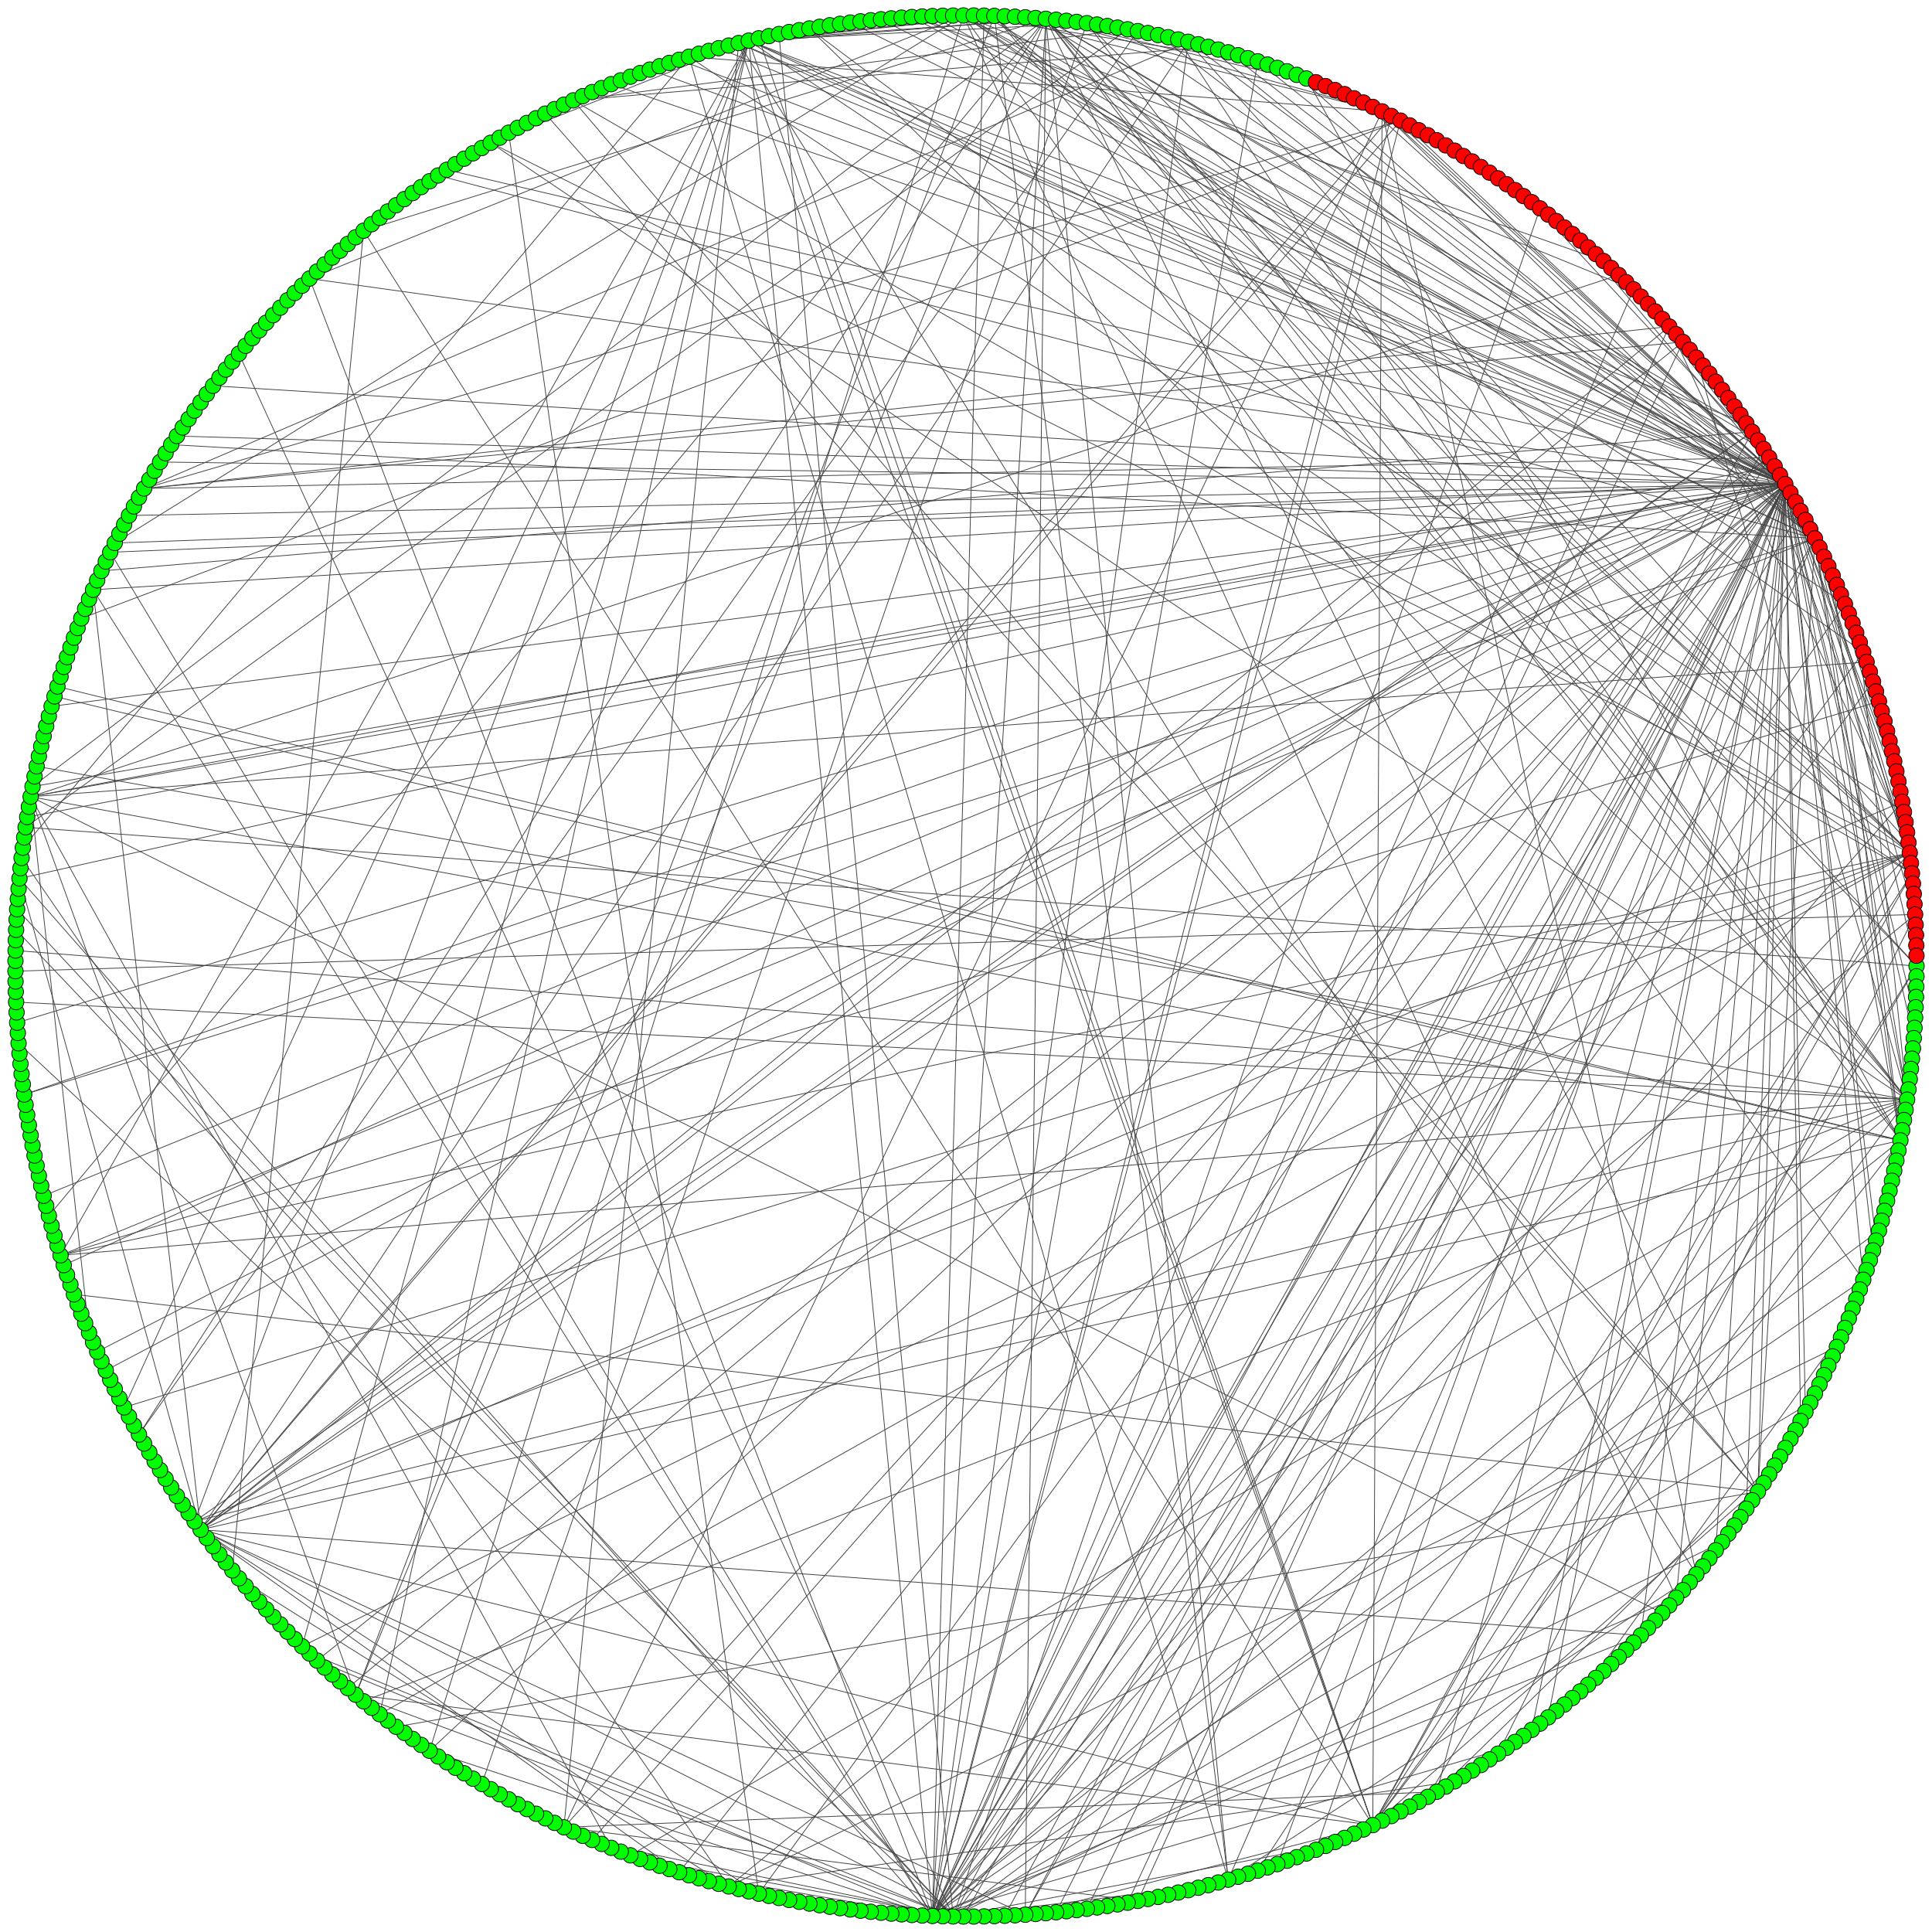
\includegraphics[width=\columnwidth]{community-circular.png}}
 \caption{Example of a figure caption.}
\end{figure}

\begin{figure}[htbp]
 \centerline{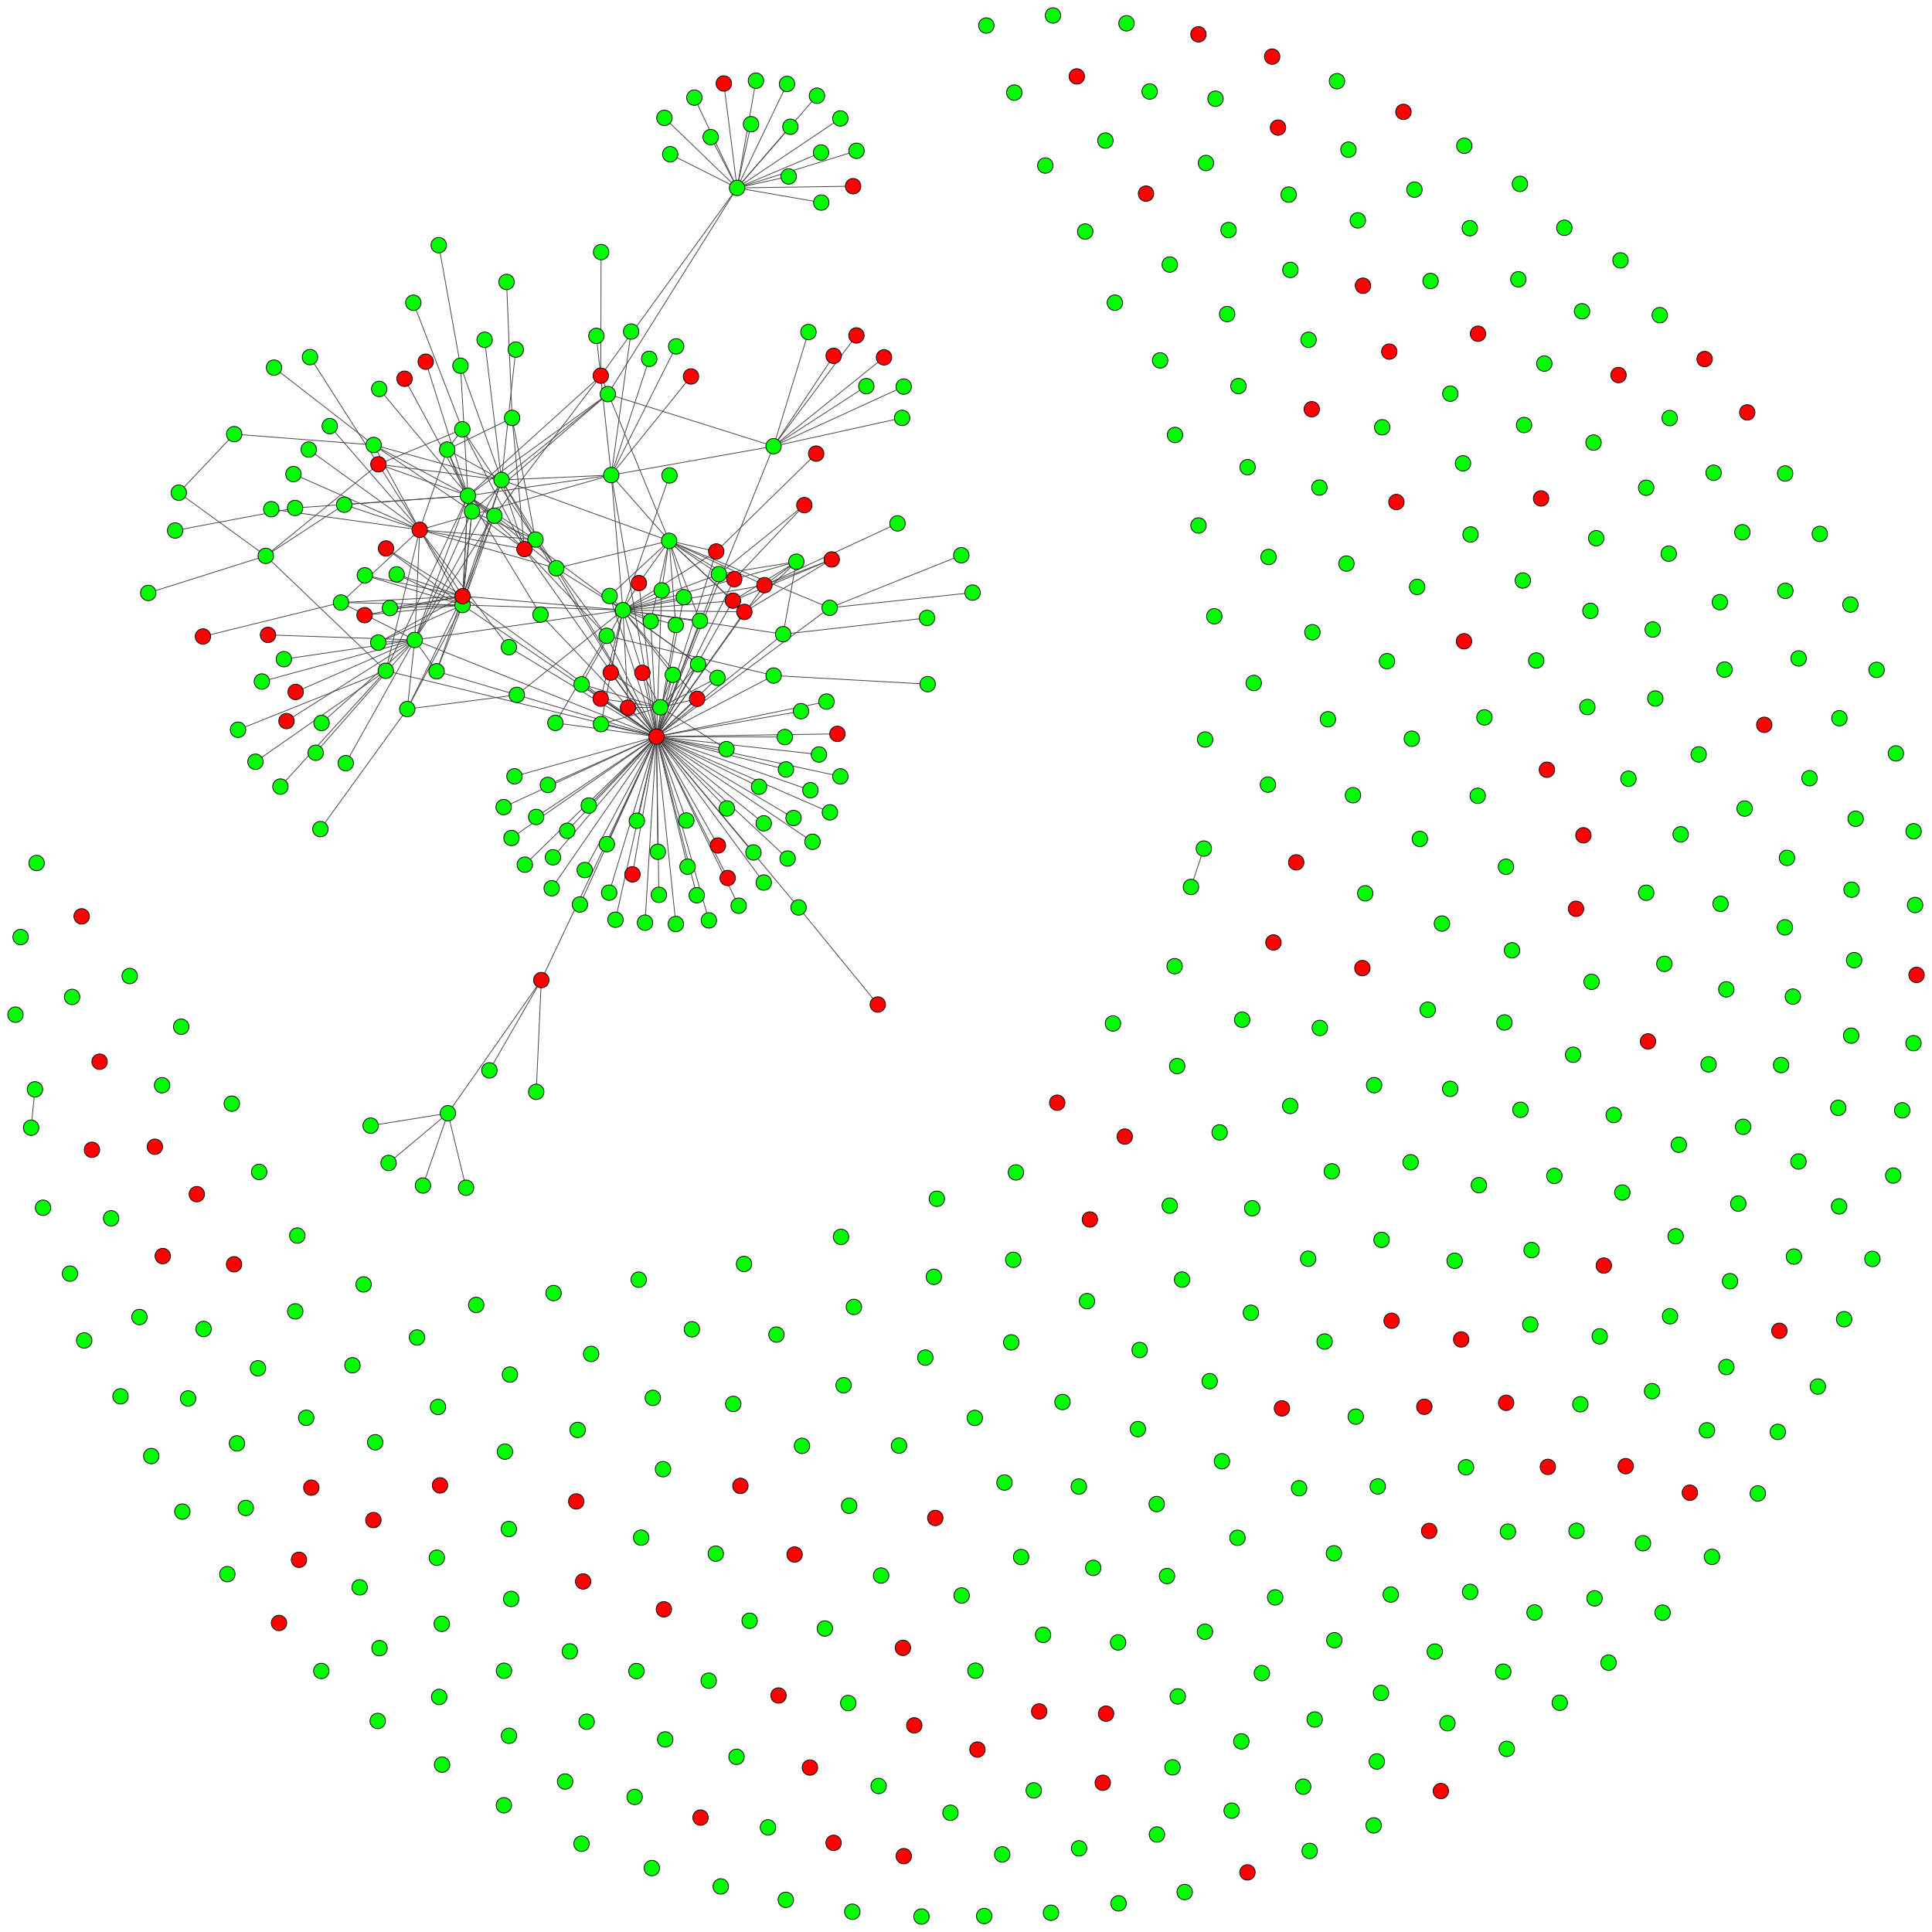
\includegraphics[width=\columnwidth]{community_fr.png}}
 \caption{Example of a figure caption.}
\end{figure}

Within each cluster, all the websites should have something in common. The results show that LPA can detect super niche communities. Some examples of this are the Indigenous Canadian community, the Pacific-Northwest Motorcycle community, and the French Astrophotography community. These communities are mostly still up, with very few dead links. In line with the goals of this project, the algorithm was able to successfully find some online ghost towns. One example of this is what looks like the Chinese Gambling website community. None of the fourteen websites in this community are still up. It is possible that these websites were terminated or reported.

\section{Results and Findings}
LPA marks similar websites with connections and if dive into the content of graph, 
clusters of communities can be observed. 
Firstly, 
no surprise are the communities of big tech companies:
At Figure \ref{fig:tech}, few of these largest communities are ventered by facebook.com, weibo.com dahucap.com and so on.

\begin{figure}[htbp]
 \centerline{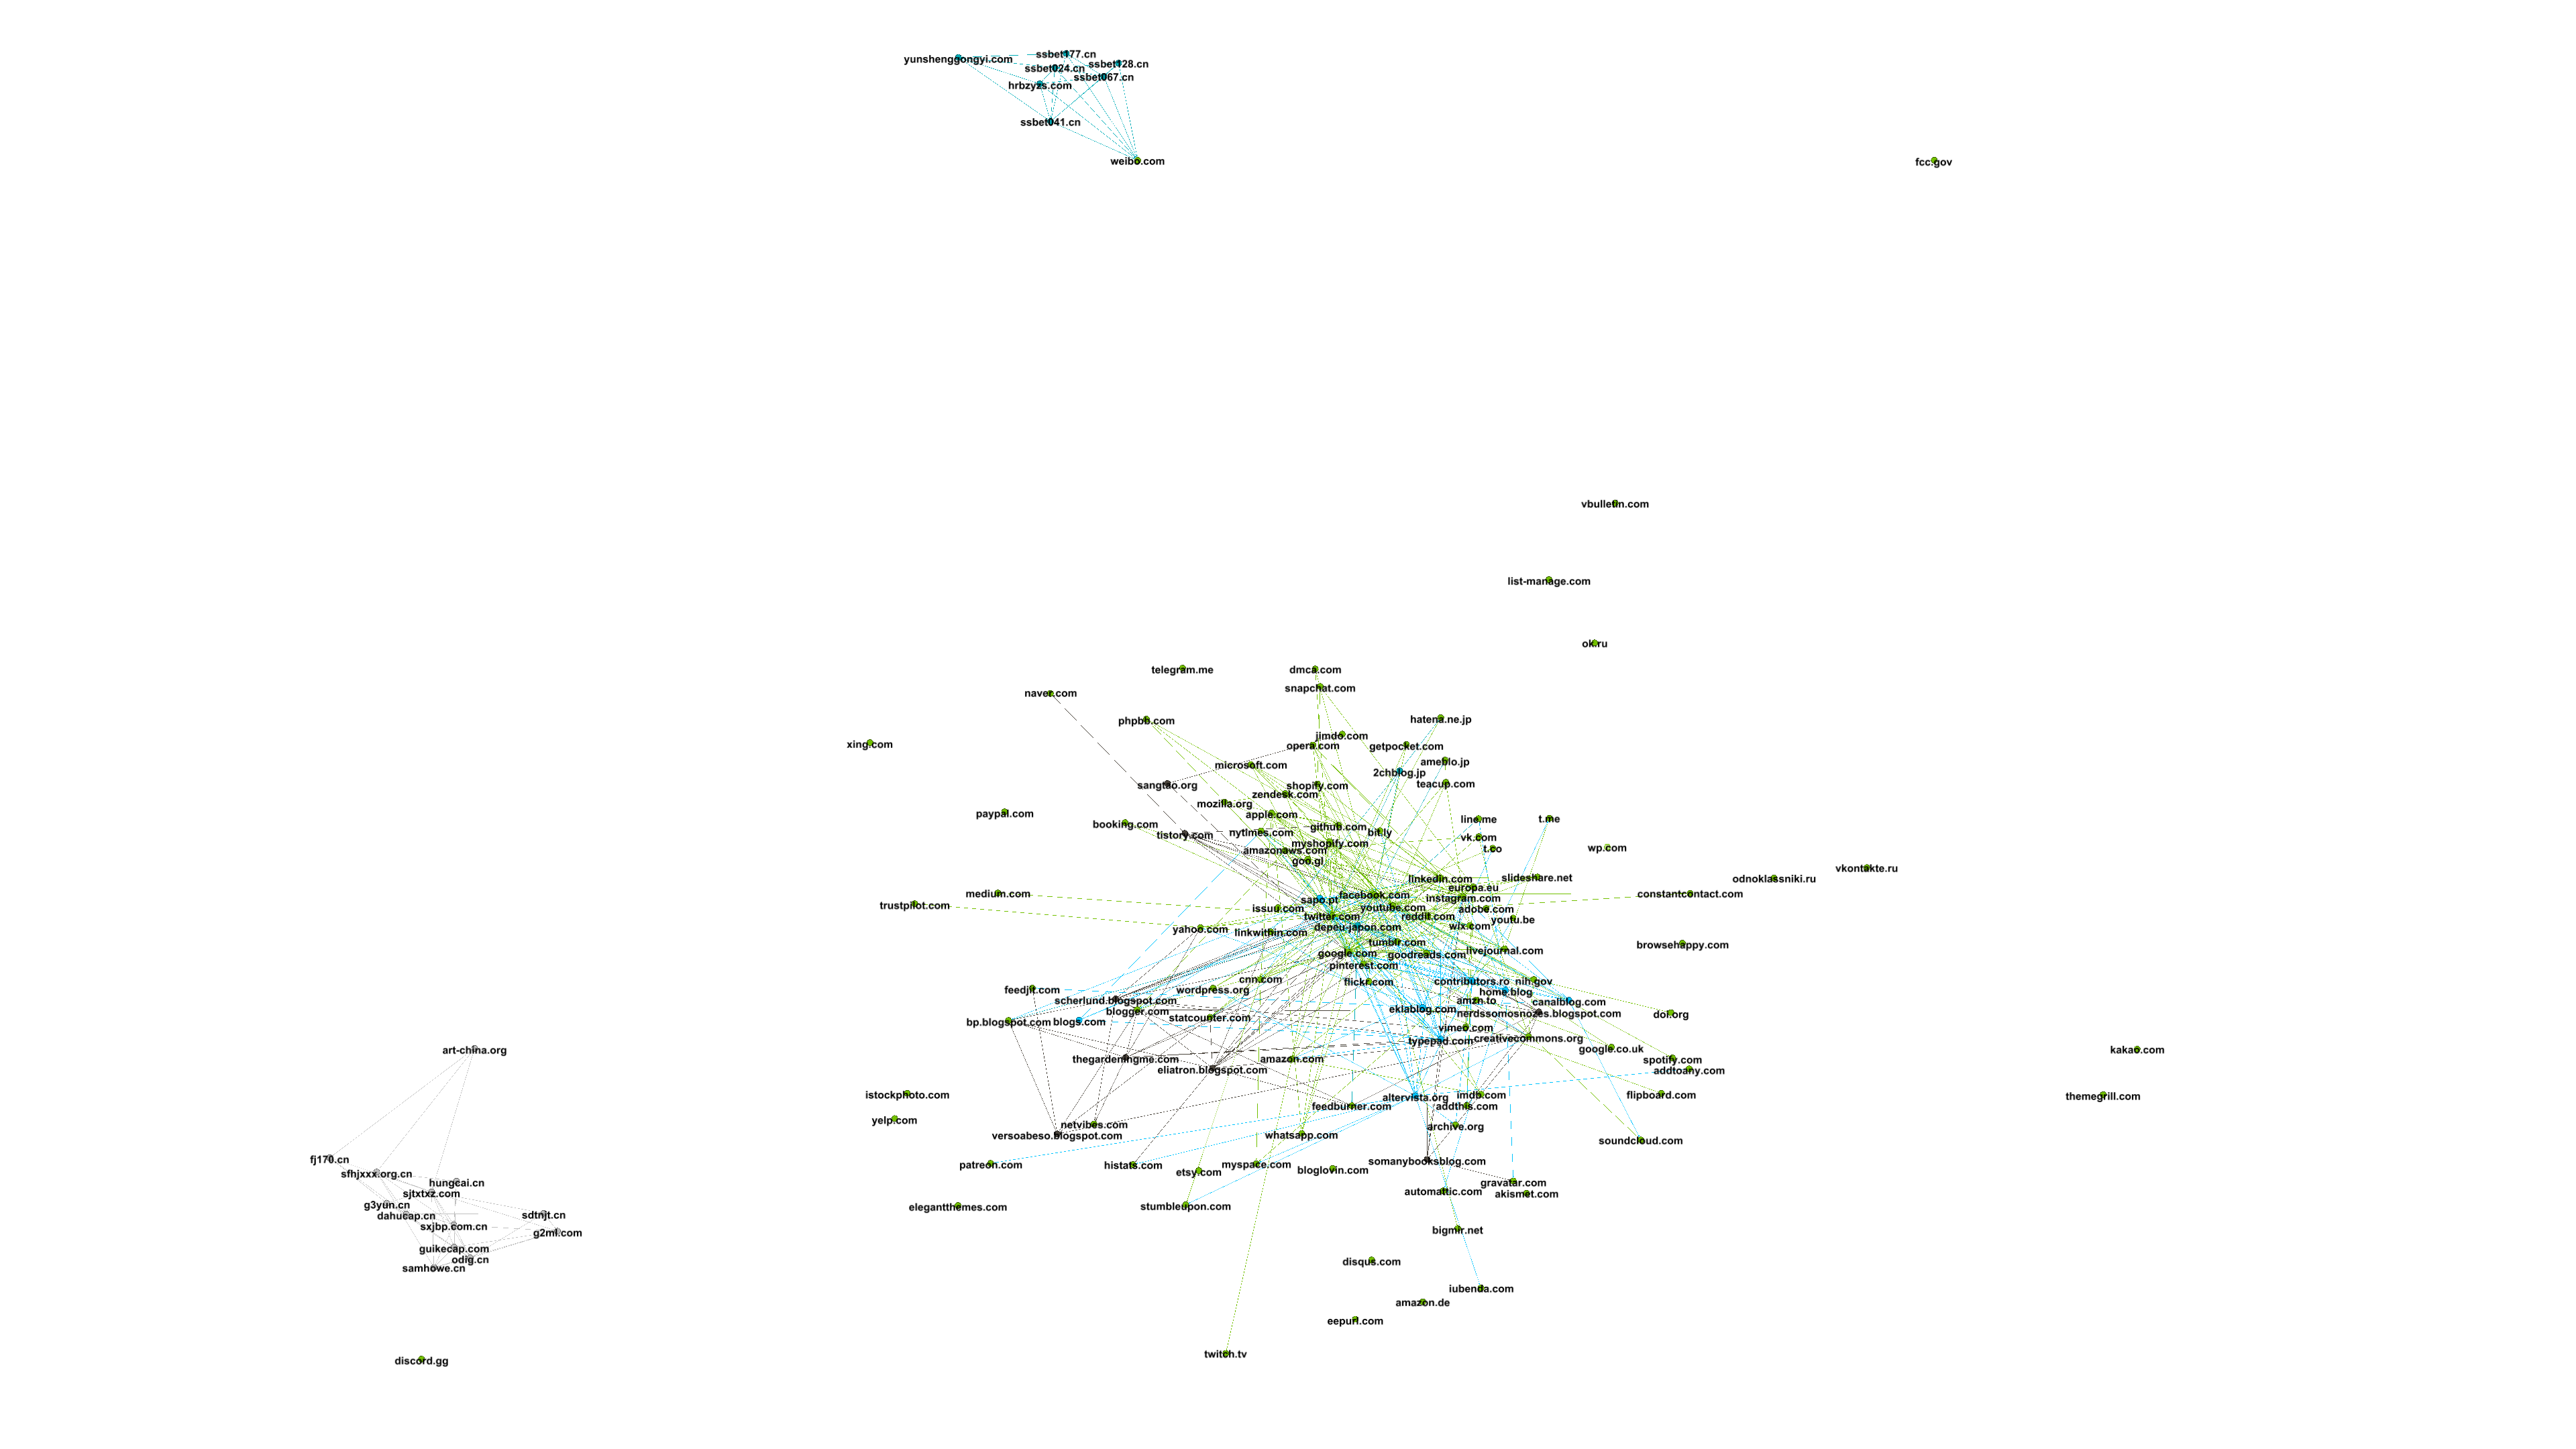
\includegraphics[width=\columnwidth]{figs/Huge.png}}
 \caption{An overview of biggest communities of LPA result}
\end{figure}

\begin{figure}[htbp]
 \centerline{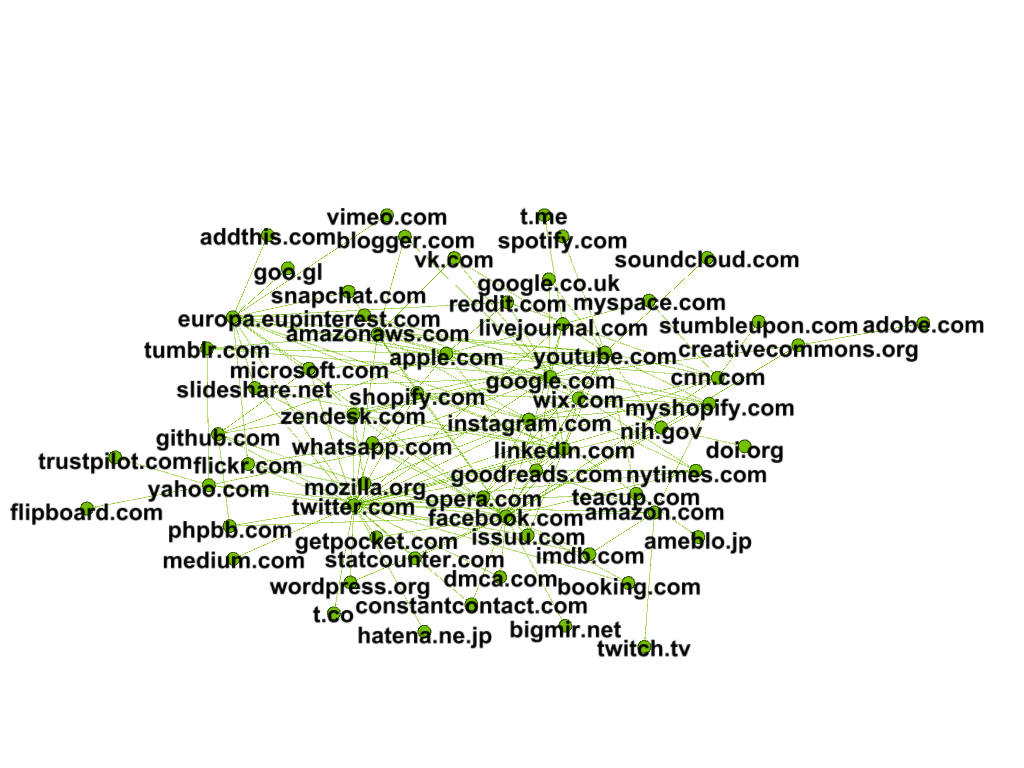
\includegraphics[width=\columnwidth]{figs/google.png}}
 \caption{A zoomed in view of the largest community}
 \label{fig:tech}
\end{figure}
Next up are the smaller communities shown in Figure \ref{fig:small groups}, 
note that they are highly uniform and are very specific.

\begin{figure}
    \centering
    \subfigure[]{
\includegraphics[width=0.24\textwidth]{figs/motor.png}} 
    \subfigure[]{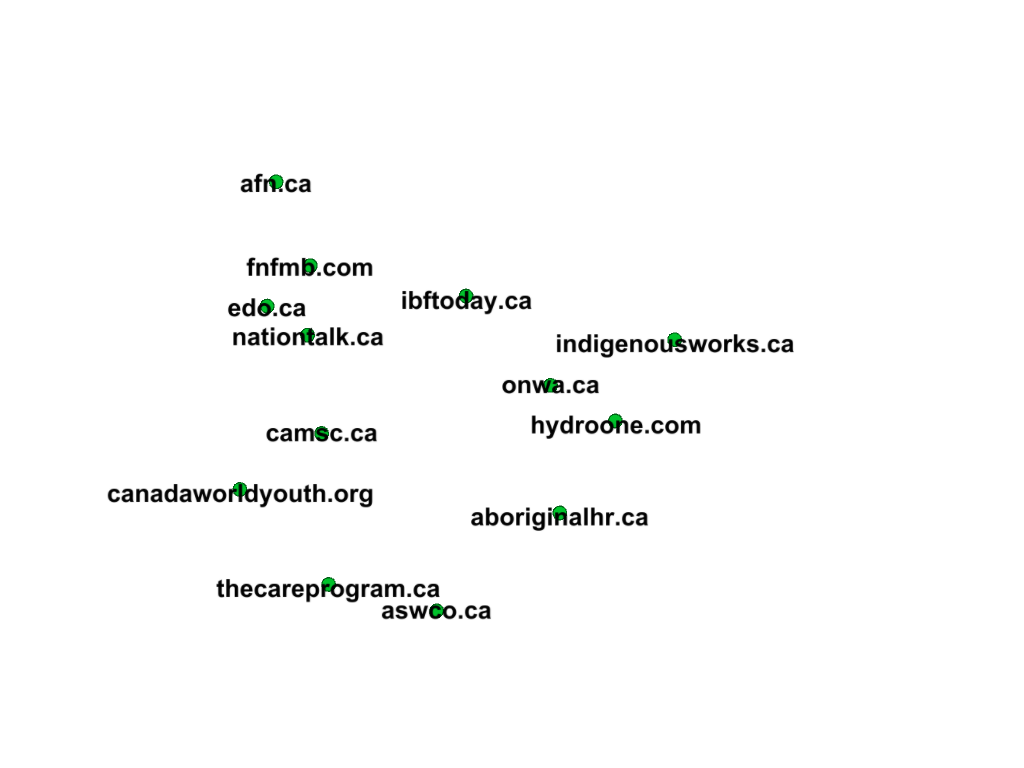
\includegraphics[width=0.24\textwidth]{figs/indigenous.png}} 
    \subfigure[]{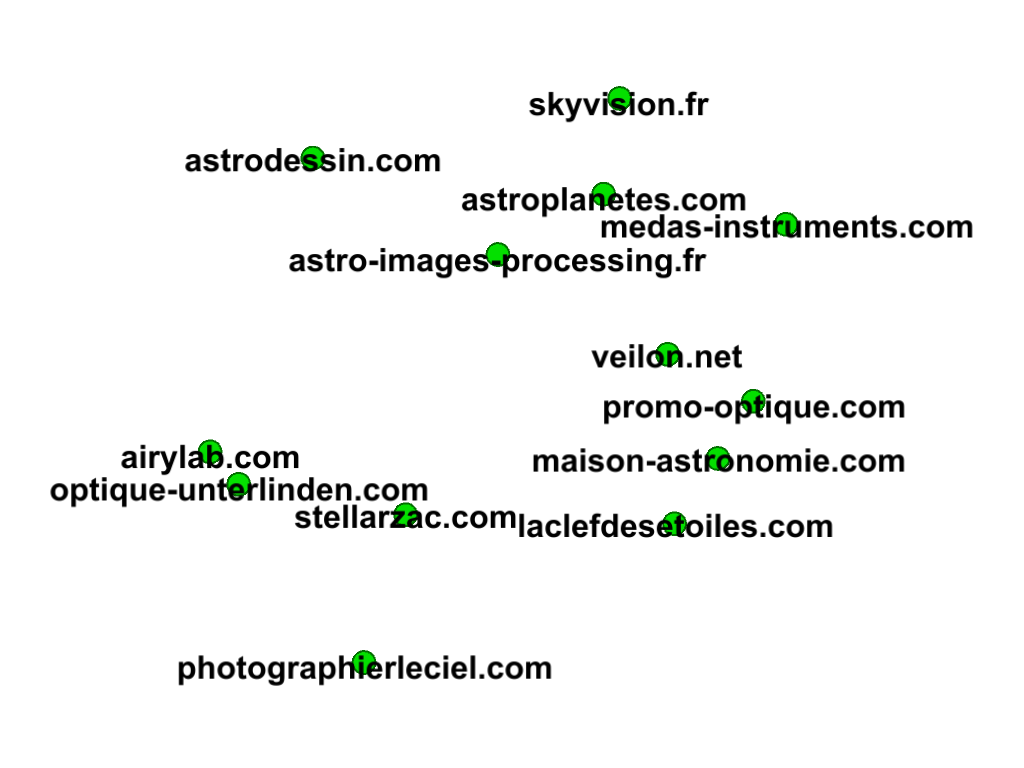
\includegraphics[width=0.24\textwidth]{figs/astro.png}}
    \caption{(a)Northwestern Motorcycle Group (b)Canadian Indigenous Group (c) French Astronomy Photography Group}
    \label{fig:small groups}
\end{figure}

To find out which community is still active and which ones are dead, 
a series targeted community HTTP requests was made to the web hosts. 
The results of the pings are astonishing and yet satisfying: 
Web pages with higher Pageranks\cite{ilprints422} are more likely to be alive whereas web sites with low Pagerank are prone to death.

Some of the websites that are shady has a shorter life expectancy, 
for communities such as Figure \ref{fig:dead}.
seeing them through web cache it is easy to tell that they are mostly related with online gamble industry. 
As most of the gambling websites are illegal and aims to scam innocent people, 
it is safe to infer that the phishing websites are expected to be dead very soon as they serve only one purpose: 
to scam people. 
As they get reported trough time and as the web indexing company finds out, 
the whole scamming community is likely to be eliminated.

\begin{figure}[!h]
 \centerline{
\includegraphics[width=\columnwidth]{figs/07after.png}}
 \caption{Scamming Community} 
 \label{fig:dead}
\end{figure}

\section{Conclusion}
\lipsum[2-4]


\bibliographystyle{IEEEtran}
\bibliography{citations}
\end{document}